\section{Gui  Class Reference}
\label{classGui}\index{Gui@{Gui}}
A generic class for designing graphical user interfaces (GUIs). 


{\tt \#include $<$gui.h$>$}

Inheritance diagram for Gui::\begin{figure}[H]
\begin{center}
\leavevmode
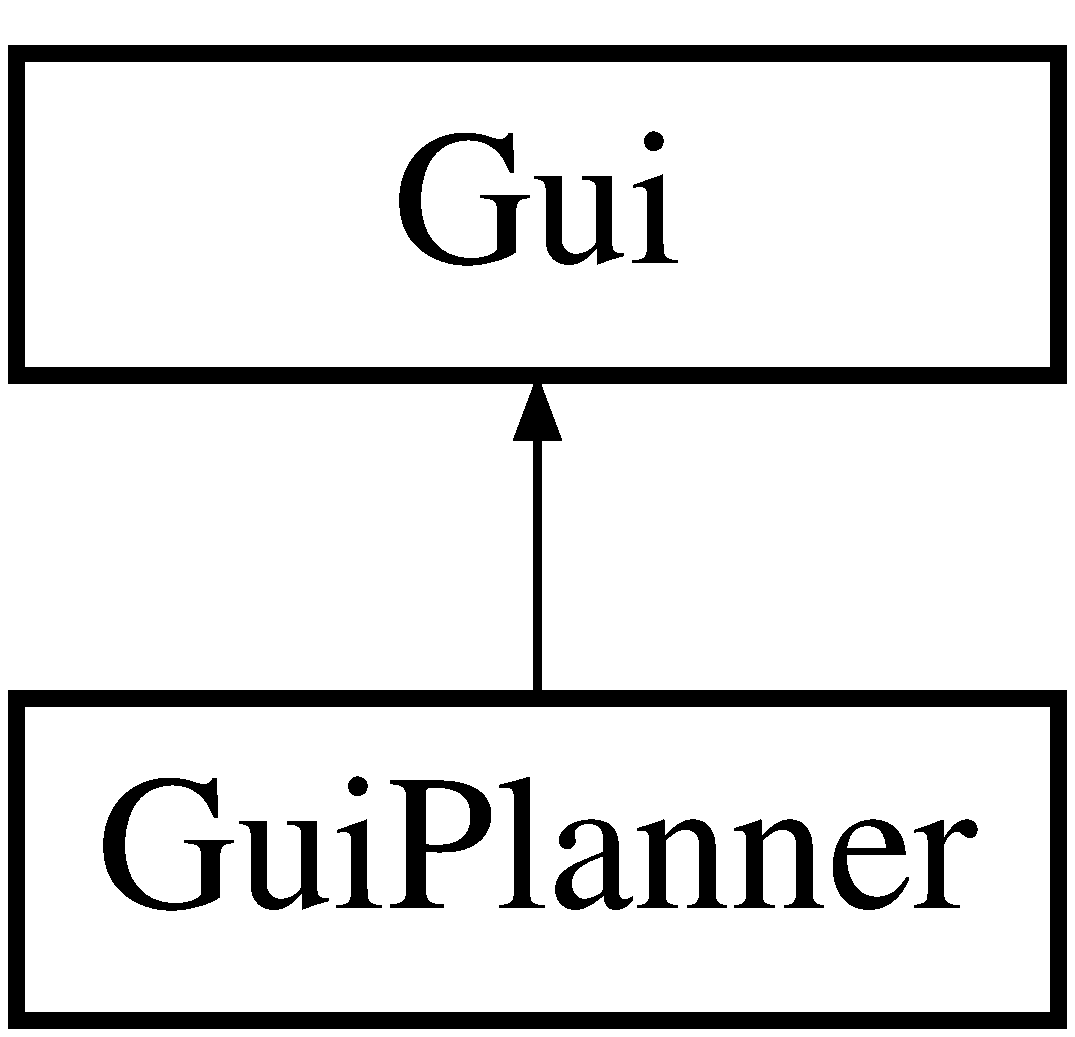
\includegraphics[height=2cm]{classGui}
\end{center}
\end{figure}
\subsection*{Public Methods}
\begin{CompactItemize}
\item 
{\bf Gui} ({\bf Render} $\ast$render)
\begin{CompactList}\small\item\em The window.\item\end{CompactList}\item 
virtual {\bf $\sim$Gui} ()
\item 
virtual void {\bf Start} ()
\begin{CompactList}\small\item\em Start running the Gui.\item\end{CompactList}\item 
virtual void {\bf Handle\-Events} ()=0
\begin{CompactList}\small\item\em Process any IO events (may be used by {\bf Render} {\rm (p.\,\pageref{classRender})}).\item\end{CompactList}\item 
virtual void {\bf Button\-Handle} (int b)
\begin{CompactList}\small\item\em Figure out what actions to take based on menu choices.\item\end{CompactList}\end{CompactItemize}
\subsection*{Public Attributes}
\begin{CompactItemize}
\item 
{\bf Render}$\ast$ {\bf R}
\item 
bool {\bf Finished}
\begin{CompactList}\small\item\em Set to true if you want to main loop to terminate.\item\end{CompactList}\end{CompactItemize}
\subsection*{Protected Methods}
\begin{CompactItemize}
\item 
virtual void {\bf Create\-Window} ()
\begin{CompactList}\small\item\em Make the menu window.\item\end{CompactList}\item 
virtual void {\bf Init} ()
\begin{CompactList}\small\item\em Initialize Gui and {\bf Render} {\rm (p.\,\pageref{classRender})}.\item\end{CompactList}\item 
virtual void {\bf Main\-Loop} ()
\begin{CompactList}\small\item\em The main event processing loop.\item\end{CompactList}\end{CompactItemize}
\subsection*{Protected Attributes}
\begin{CompactItemize}
\item 
string {\bf File\-Path}
\end{CompactItemize}


\subsection{Detailed Description}
A generic class for designing graphical user interfaces (GUIs).

The graphical user interface (GUI) is designed as a hierarchy of classes to enable specific user interfaces to be designed for a variety of different motion strategy problems and planning algorithms. Currently, there is one derived class which serves as the GUI for all of the {\bf RRT} {\rm (p.\,\pageref{classRRT})}-based planners. Each instance of Gui includes an instance of an {\bf RRT} {\rm (p.\,\pageref{classRRT})} {\bf Planner} {\rm (p.\,\pageref{classPlanner})} class and an instance of a {\bf Render} {\rm (p.\,\pageref{classRender})} class. Using this design, the same basic GUI design can be used, regardless of the particular rendering methods. 



\subsection{Constructor \& Destructor Documentation}
\index{Gui@{Gui}!Gui@{Gui}}
\index{Gui@{Gui}!Gui@{Gui}}
\subsubsection{\setlength{\rightskip}{0pt plus 5cm}Gui::Gui ({\bf Render} $\ast$ {\em render})}\label{classGui_a0}


The window.

\index{Gui@{Gui}!~Gui@{$\sim$Gui}}
\index{~Gui@{$\sim$Gui}!Gui@{Gui}}
\subsubsection{\setlength{\rightskip}{0pt plus 5cm}Gui::$\sim$Gui ()\hspace{0.3cm}{\tt  [inline, virtual]}}\label{classGui_a1}




\subsection{Member Function Documentation}
\index{Gui@{Gui}!ButtonHandle@{ButtonHandle}}
\index{ButtonHandle@{ButtonHandle}!Gui@{Gui}}
\subsubsection{\setlength{\rightskip}{0pt plus 5cm}void Gui::Button\-Handle (int {\em b})\hspace{0.3cm}{\tt  [inline, virtual]}}\label{classGui_a4}


Figure out what actions to take based on menu choices.



Reimplemented in {\bf Gui\-Planner} {\rm (p.\,\pageref{classGuiPlanner_a1})}.\index{Gui@{Gui}!CreateWindow@{CreateWindow}}
\index{CreateWindow@{CreateWindow}!Gui@{Gui}}
\subsubsection{\setlength{\rightskip}{0pt plus 5cm}void Gui::Create\-Window ()\hspace{0.3cm}{\tt  [inline, protected, virtual]}}\label{classGui_b0}


Make the menu window.

\index{Gui@{Gui}!HandleEvents@{HandleEvents}}
\index{HandleEvents@{HandleEvents}!Gui@{Gui}}
\subsubsection{\setlength{\rightskip}{0pt plus 5cm}void Gui::Handle\-Events ()\hspace{0.3cm}{\tt  [pure virtual]}}\label{classGui_a3}


Process any IO events (may be used by {\bf Render} {\rm (p.\,\pageref{classRender})}).



Reimplemented in {\bf Gui\-Planner} {\rm (p.\,\pageref{classGuiPlanner_a0})}.\index{Gui@{Gui}!Init@{Init}}
\index{Init@{Init}!Gui@{Gui}}
\subsubsection{\setlength{\rightskip}{0pt plus 5cm}void Gui::Init ()\hspace{0.3cm}{\tt  [protected, virtual]}}\label{classGui_b1}


Initialize Gui and {\bf Render} {\rm (p.\,\pageref{classRender})}.



Reimplemented in {\bf Gui\-Planner} {\rm (p.\,\pageref{classGuiPlanner_b0})}.\index{Gui@{Gui}!MainLoop@{MainLoop}}
\index{MainLoop@{MainLoop}!Gui@{Gui}}
\subsubsection{\setlength{\rightskip}{0pt plus 5cm}void Gui::Main\-Loop ()\hspace{0.3cm}{\tt  [protected, virtual]}}\label{classGui_b2}


The main event processing loop.

\index{Gui@{Gui}!Start@{Start}}
\index{Start@{Start}!Gui@{Gui}}
\subsubsection{\setlength{\rightskip}{0pt plus 5cm}void Gui::Start ()\hspace{0.3cm}{\tt  [virtual]}}\label{classGui_a2}


Start running the Gui.



\subsection{Member Data Documentation}
\index{Gui@{Gui}!FilePath@{FilePath}}
\index{FilePath@{FilePath}!Gui@{Gui}}
\subsubsection{\setlength{\rightskip}{0pt plus 5cm}string Gui::File\-Path\hspace{0.3cm}{\tt  [protected]}}\label{classGui_n0}


\index{Gui@{Gui}!Finished@{Finished}}
\index{Finished@{Finished}!Gui@{Gui}}
\subsubsection{\setlength{\rightskip}{0pt plus 5cm}bool Gui::Finished}\label{classGui_m1}


Set to true if you want to main loop to terminate.

\index{Gui@{Gui}!R@{R}}
\index{R@{R}!Gui@{Gui}}
\subsubsection{\setlength{\rightskip}{0pt plus 5cm}{\bf Render} $\ast$ Gui::R}\label{classGui_m0}




The documentation for this class was generated from the following files:\begin{CompactItemize}
\item 
{\bf gui.h}\item 
{\bf gui.C}\end{CompactItemize}
